\documentclass[usenames,dvipsnames]{beamer}
%-------------------------------------------------------
% THEME SETTINGS
%-------------------------------------------------------
\usetheme[progressstyle=movingCircCnt]{Feather}
\setbeamercolor{Feather}{fg=black!30,bg=black}
\setbeamercolor{structure}{fg=black}
\setbeamercolor{block body example}{bg=black!5!white}
\setbeamercolor{block title example}{fg=white,bg=black!40!white}


\usepackage{amsmath,amssymb,amsfonts}
\usepackage{cite}
\usepackage{multirow}
\usepackage{booktabs}
\usepackage{hhline}
\usepackage{multicol}
%\usepackage{showframe}

\usepackage{tikz}
%\usetikzlibrary{patterns}
\usetikzlibrary{patterns,arrows,decorations.pathmorphing,backgrounds,shadows,positioning,fit,shapes,matrix,calc,shapes.multipart,arrows.meta}
\usepackage[simplified]{pgf-umlcd}
\usepackage{xpatch} % Needed for patching pgf-umlcd
\usepackage{xparse} % Needed for patching pgf-umlcd
\usepackage{color,soul} % for \hl
\definecolor{dark-yellow}{RGB}{219, 212, 143}
\definecolor{dark-green}{RGB}{36,84,36}
\definecolor{my-gray}{gray}{0.85}
\sethlcolor{dark-yellow}



\usepackage{wrapfig}
\usepackage{listings}
\usepackage{adjustbox}
\usepackage{graphicx}
\usepackage{caption}
\usepackage{multirow}
\usepackage{subcaption}
\usepackage{stmaryrd}
\usepackage{hyperref}
\usepackage{float}
\usepackage{textcomp}
\usepackage{tikz-qtree,tikz-qtree-compat}

\newcommand*{\emphColorSlide}[1]{\textcolor{ForestGreen}{\textbf{#1}}}
\newcommand*{\emphSlide}[1]{\textcolor{ForestGreen}{\textbf{#1}}}

\newcommand*{\lowEmph}[1]{\textcolor{NavyBlue}{\textbf{#1}}}
\newcommand*{\subt}{\textcolor{NavyBlue}{\textbf{<:}}}
\newcommand*{\supt}{\textcolor{NavyBlue}{\textbf{:>}}}



\newcommand{\dataflow}{data-flow}
\newcommand{\Dataflow}{Data-flow}
\newcommand{\code}[1]{\texttt{\lstinline[basicstyle=\normalsize\ttfamily,identifierstyle={\normalsize},commentstyle={\normalsize\itshape},keywordstyle={\normalsize\bfseries},ndkeywordstyle={\normalsize},stringstyle={\normalsize\ttfamily},numberstyle={\normalsize}]!#1!}}
\newcommand{\CFG}{CFG}
\newcommand{\intraj}{\emphColorSlide{\textsc{Intra}J}}
\newcommand{\intrajs}{\emphColorSlide{\textsc{IntraJ}}}
\newcommand{\intracfgs}{\emphColorSlide{\textsc{IntraCFG}}}
\newcommand{\jastaddjintraflow}{\textsc{jastaddj-intraflow}}
\newcommand{\jji}{\code{JJI}}
\newcommand{\jastadd}{\textsc{JastAdd}}
\newcommand{\extendj}{\textsc{ExtendJ}}
\newcommand{\cG}{\mathcal{G}}
\newcommand{\cV}{\mathcal{V}}
\newcommand{\cE}{\rightarrowtail}
\newcommand{\cP}{\mathcal{P}}
\newcommand{\cM}{\mathcal{M}}


\newcommand{\mSyn}{\ensuremath{\uparrow}}
\newcommand{\mInh}{\ensuremath{\downarrow}}
\newcommand{\mHOA}{\ensuremath{\rightarrow}}
\newcommand{\mColl}{\ensuremath{\square}}
\newcommand{\mCirc}{\ensuremath{\circlearrowleft}}

\newcommand{\Abase}[1]{\textcolor{ATGsym}{\mbox{\umlcode{#1}}}}
\newcommand{\Asyn}[1]{\textcolor{ATGsym}{\mbox{\mSyn{}\umlcode{#1}}}}
\newcommand{\Ainh}[1]{\textcolor{ATGsym}{\mbox{\mInh{}\umlcode{#1}}}}
\newcommand{\Ahoa}[1]{\textcolor{ATGsym}{\mbox{\mHOA{}\umlcode{#1}}}}
\newcommand{\Acoll}[1]{\textcolor{ATGsym}{\mbox{\mColl{}\umlcode{#1}}}}
\newcommand{\Acirc}[1]{\textcolor{ATGsym}{\mbox{\mCirc{}\umlcode{#1}}}}

\newcommand{\umlcode}[1]{\textrm{#1}}  % Style of code used in UML fragments
\newcommand{\astnodestyle}{\ttfamily\color{magenta}}
\newcommand{\astnode}[1]{\texttt{\textcolor{magenta}{#1}}}  % Style used for AST node types

\newcommand{\ASTUnrestricted}{AST-unrestricted}
\newcommand{\ParentFirst}{Parent-First}

\newcommand{\project}[1]{\textsc{#1}}
\newcommand{\tool}[1]{\textsc{#1}}

% can't get fbox to work reliably in the UML code, and adjustbox and nested \tikz don't work at all
%\newcommand{\dfapi}{\textsf{\setlength{\fboxsep}{0pt}\fcolorbox{blue}{white}{df-api}}}
\newcommand{\dfapi}{\textbf{\textcolor{black}{[df-api]}}}
\newcommand{\nameapi}{\textbf{\textcolor{black}{[name-api]}}}

\newcommand{\frameworkname}{\textsc{Intra}CFG}
\newcommand{\intracfg}{\textsc{\frameworkname}}

\newcommand{\node}{\mathsf{n}}
\newcommand{\Null}{\mathtt{NULL}}
\newcommand{\Notnull}{\mathtt{NOTNULL}}
\newcommand{\gen}{\mathtt{gen}}
\renewcommand{\kill}{\mathtt{kill}}

\newcommand{\In}{\mathtt{in}}
\newcommand{\Out}{\mathtt{out}}
\newcommand{\Use}{\mathtt{use}}
\newcommand{\Def}{\mathtt{def}}
\newcommand{\tf}{f_t}
\newcommand{\mCi}[1]{ { \textcolor{black!30}{\tiny \pm\text{#1}}}}%Condifdence interval

\newcommand{\CR}[1]{\textbf{[}\textcolor{blue!60!black}{\textbf{CR:} #1}\textbf{]}}
\newcommand{\Ckw}[1]{\texttt{\textbf{#1}}}
\newcommand{\auxlabel}[1]{{\scriptsize{$\textrm{\texttt{#1}}$}}}
\newcommand{\auxlabeli}[2]{{\scriptsize{$\textrm{\texttt{#2}}_{#1}$}}}
\newcommand{\auxlabelbox}[1]{\tikz[baseline=-0.7ex] \node[rectangle, minimum width=0, thin, draw, rounded corners, fill=white, inner sep=2pt, outer sep=0pt] (N) {\auxlabel{#1}};}
\newcommand{\auxlabelboxhoa}[1]{\tikz[baseline=-0.7ex] \node[rectangle, dashed,minimum width=0, thin, draw, rounded corners, fill=white, inner sep=2pt, outer sep=0pt] (N) {\auxlabel{#1}};}

%\newcommand{\auxlabelboxi}[2]{\tikz \node[rectangle, minimum width=0, thin, draw, rounded corners, fill=white] {\auxlabeli{#1}{#2}};}

\newcommand{\Prod}{::=}
\newcommand{\terminal}[1]{\textcolor{green!50!black}{\textit{#1}}}
\newcommand{\vmetavar}[1]{\textcolor{cyan!30!black}{\textsf{\textbf{#1}}}}
\newcommand{\vcode}[1]{\textsf{\textcolor{green!35!black}{{#1}}}}
\newcommand{\vterminal}[1]{\vcode{#1}}
\newcommand{\nta}[1]{\ensuremath{\textit{#1}}}
\newcommand{\tuple}[1]{\ensuremath{\langle #1 \rangle}}
\newcommand{\nt}[1]{\ensuremath{\tuple{\hspace{-0.02cm}\nta{#1}\hspace{0.02cm}}}}
\newcommand{\VB}{\ |\ }
\newcommand{\Gcomment}[1]{\textrm{\textcolor{black!50!white}{({#1})}}}
\newcommand{\sem}[1]{\ensuremath{\llbracket #1 \rrbracket}}
%\newcommand{\semNPA}[1]{\ensuremath{\sem{#1}_{\textit{NPA}}}}
\newcommand{\semNPA}[1]{\ensuremath{\sem{#1}}}

\newcommand{\listingsfontsize}{\scriptsize}

\newcommand{\NAmark}{\multicolumn{1}{c}{\textcolor{black!40!white}{-}}}
\newcommand{\NAmarkR}{\multicolumn{1}{c|}{\textcolor{black!40!white}{-}}}
\newcommand{\Tcenter}[1]{\multicolumn{1}{c}{#1}}
\newcommand{\TcenterR}[1]{\multicolumn{1}{c|}{#1}}
\newcommand{\succarrow}{\tikz[baseline=-0.7ex] \draw[succarrow, thick, -{Stealth[scale=0.9, inset=0pt, angle'=45]}] (0,0) -- (0.3,0.0);}

\colorlet{hlgreen}{green}
\colorlet{hlorange}{orange}
\colorlet{hlgreenhalf}{green!50!white}
\colorlet{hlorangehalf}{orange!50!white}
\colorlet{npagrey}{gray!10!white}

\DeclareRobustCommand{\hlgreen}[1]{{\sethlcolor{hlgreenhalf}\hl{#1}}}
\DeclareRobustCommand{\hlorange}[1]{{\sethlcolor{hlorangehalf}\hl{#1}}}

\definecolor{ATGsym}{HTML}{206010}

\definecolor{SQ}{HTML}{0080ff}
\definecolor{JJI}{HTML}{ff0080}
\definecolor{IJnonH}{HTML}{004010}
\definecolor{IJH}{HTML}{00ff20}

\definecolor{succarrow}{HTML}{4e90e2}	% adapted from RunningExample.tex

\definecolor{lightblue}{HTML}{006699}		%#006699
\definecolor{lightgreen}{HTML}{669900}		%#669900
\lstdefinelanguage{JastAdd}{
  %keyword1&2&6
  morekeywords = [1]{class, extends, private, void,new},
  %keyword3
  morekeywords = [2]{this,null}, %JASTADD keywords
  %keyword4
  morekeywords = [3]{return}, %ASTnode typess
  %keyword5
  morekeywords = [4]{},
  keywordstyle = [1]\color{lightblue},
  keywordstyle = [2]\color{lightgreen},
%  keywordstyle = [1]\bfseries,
%  keywordstyle = [2]\bfseries,
  keywordstyle = [3]\astnodestyle,
  keywordstyle = [4]\color{orange},
  sensitive = true,
  morecomment = [l]{//},
  morecomment = [s]{/*}{*/},
  morecomment = [s]{/**}{*/},
  commentstyle = \color{gray},
  morestring = [b]",
  morestring = [b]',
  stringstyle = \color{purple}
}
\lstset{
  backgroundcolor =\color{npagrey},
  basicstyle=\listingsfontsize\ttfamily,
  identifierstyle={\listingsfontsize},
  commentstyle={\listingsfontsize\itshape},
  keywordstyle={\listingsfontsize\bfseries},
  ndkeywordstyle={\listingsfontsize},
  stringstyle={\listingsfontsize\ttfamily},
  frame={tb},
  breaklines=true,
  breakatwhitespace=true, %To avoid linebreaks between \code{} and comma.
  columns=[l]{fullflexible},
  numbers=none,
  numberstyle={\listingsfontsize},
  stepnumber=1,
  mathescape,
	escapeinside     = {!}{!}, %General escape does not seem to work in lstinline/GH.
}

\makeatletter
\pgfdeclareshape{topbottombox}{
  \inheritsavedanchors[from=rectangle]
  \inheritanchorborder[from=rectangle]
  \inheritanchor[from=rectangle]{center}
  \inheritanchor[from=rectangle]{base}
  \inheritanchor[from=rectangle]{north}
  \inheritanchor[from=rectangle]{north east}
  \inheritanchor[from=rectangle]{east}
  \inheritanchor[from=rectangle]{south east}
  \inheritanchor[from=rectangle]{south}
  \inheritanchor[from=rectangle]{south west}
  \inheritanchor[from=rectangle]{west}
  \inheritanchor[from=rectangle]{north west}
  \backgroundpath{
    %  store lower right in xa/ya and upper right in xb/yb
    \southwest \pgf@xa=\pgf@x \pgf@ya=\pgf@y
    \northeast \pgf@xb=\pgf@x \pgf@yb=\pgf@y
    \pgfpathmoveto{\pgfpoint{\pgf@xa}{\pgf@ya}}
    \pgfpathlineto{\pgfpoint{\pgf@xb}{\pgf@ya}}
    \pgfpathmoveto{\pgfpoint{\pgf@xa}{\pgf@yb}}
    \pgfpathlineto{\pgfpoint{\pgf@xb}{\pgf@yb}}
 }
}
\makeatother


% Patch UML package pgf-umlcd to be able to write abstract grammar as class name.
\ExplSyntaxOn
\NewDocumentCommand{\defineclassname}{m}
 {
  \tl_set:Nn \umlcdClassName { #1 }
  \tl_set_eq:NN \umlcdClassNameString \umlcdClassName
  \tl_replace_all:Nfn \umlcdClassName { \char_generate:nn { `_ } { 8 } } { \_\kern1pt }
 }
\cs_generate_variant:Nn \tl_replace_all:Nnn { Nf }
\ExplSyntaxOff
\xpatchcmd{\classAndInterfaceCommon}
 {\def\umlcdClassName}
 {\defineclassname}
 {}{}
\xpatchcmd{\endclass}
 {(\umlcdClassName)}
 {(\umlcdClassNameString)}
 {}{\ddt}
\xpatchcmd{\endinterface}
 {(\umlcdClassName)}
 {(\umlcdClassNameString)}
 {}{\ddt}
\xpatchcmd{\endabstractclass}
 {(\umlcdClassName)}
 {(\umlcdClassNameString)}
 {}{\ddt}
\xpatchcmd{\endobject}
 {(\umlcdClassName)}
 {(\umlcdClassNameString)}
 {}{\ddt}
\xpatchcmd{\endclassAndInterfaceCommon}
 {(\umlcdClassName)}
 {(\umlcdClassNameString)}
 {}{\ddt}
\xpatchcmd{\endclassAndInterfaceCommon}
 {(\umlcdClassName)}
 {(\umlcdClassNameString)}
 {}{\ddt}
\xpatchcmd{\endclassAndInterfaceCommon}
 {(\umlcdClassName)}
 {(\umlcdClassNameString)}
 {}{\ddt}

\newbool{ANON}
%\booltrue{ANON}
\boolfalse{ANON}
\newcommand{\anon}[2]
{\ifbool{ANON}{
   #1
}{
   #2
}}



\makeatletter
\renewcommand\@makefnmark{\hbox{\@textsuperscript{\usebeamercolor[fg]{footnote mark}\usebeamerfont*{footnote mark}[\@thefnmark]}}}
\renewcommand\@makefntext[1]{\@textsuperscript{\usebeamercolor[fg]{footnote mark}\usebeamerfont*{footnote mark}[\@thefnmark]}\usebeamerfont*{footnote} #1}
\makeatother

%Modify the Title display on frame
\makeatletter
\patchcmd\beamer@@tmpl@frametitle{\insertframetitle}{{\footnotesize \insertsection~\emphColorSlide{\insertsubsection}~\\} \textbf{\insertframetitle}}{}{}
\makeatother
%Add space to the footline
\makeatletter
\patchcmd{\beamer@calculateheadfoot}{\advance\footheight by 4pt}{\advance\footheight by 8pt}{}{}
\makeatother

%NO HEAD LINE
\makeatletter
\newenvironment{noheadline}{
	\setbeamertemplate{headline}[default] {}
	\setfootline
}{}
\makeatother

%Slide with  Section title
%\AtBeginSection[]{
%	\begin{noheadline}
%	\begin{frame}[noframenumbering]
%			\begin{center}
%				\large Chapter \thesection \\
%				\vspace*{1cm}
%				\centering {\usebeamerfont{title} \huge\textcolor{black}{\insertsectionhead}}
%				\vspace*{1cm}
%			\end{center}
%		\end{frame}
%	\end{noheadline}
%}


\newcommand{\setfootline}{
	\setbeamercolor{footline}{fg=white,bg=black}
	\setbeamertemplate{footline}{%
		\begin{beamercolorbox}[wd=1.0\paperwidth,left,ht=2.5ex,dp=1ex]{footline}
			\usebeamerfont{section in head/foot}%
			\hspace*{3.5ex}%
			\insertshortauthor\ |\
			\insertshorttitle
			\insertshortsubtitle
		\end{beamercolorbox}
	}
	\addtobeamertemplate{footline}{%
		\setlength\unitlength{1ex}%
		\begin{picture}(0,0)
		\put(125,3){\makebox(0,0)[bl]{
			
\includegraphics[scale=0.20]{img/scam.png}
	}}%
		\end{picture}%
	}{}
}






%-------------------------------------------------------
% INFORMATION IN THE TITLE PAGE
%-------------------------------------------------------

\subtitle[{\color{ForestGreen}\textbf{TAPL}}]
{
	\footnotesize{TAPL
}
}

\title[] % [] is optional - is placed on the bottom of the sidebar on every slide
{ % is placed on the title page
	\textsc{ On Variance-Based Subtyping for Parametric Types
	 }
}



\author[\textbf{Idriss Riouak}]
{ \emphSlide{Idriss Riouak}}

\institute[]
{\vspace{1cm}
	\textbf{Lund University}\\
	\textbf{Computer Science Department} \\
}

\date{\today}

\makeatletter
\newcommand\SoulColor{%
  \let\set@color\beamerorig@set@color
  \let\reset@color\beamerorig@reset@color}
\makeatother
\SoulColor

\begin{document}
\setfootline

%-------------------------------------------------------
% THE TITLEPAGE
%-------------------------------------------------------

{\1
\begin{frame}[plain,noframenumbering]
		\titlepage
	\end{frame}}

%-------------------------------------------------------
% BODY
%-------------------------------------------------------
\section{Introduction}
	\begin{frame}[fragile]{Overview}
		\begin{itemize}
		\item ECOOP 2002 - Atsushi \textbf{Igarashi} and Mirko \textbf{Viroli}
		\item Igarashi is one of the authors of \emphSlide{Featherweight Java}
		\item \textbf{Motivations}
		\begin{itemize}[<+->]
			\item Java's designers initially decided to avoid generic features,
			\item Only inclusive polymorphism supported by inheritance,
			\item Java5: \emphSlide{$\uparrow$} programmers' productivity; \emphSlide{$\uparrow$} readability; \emphSlide{$\uparrow$}maintainability and \emphSlide{$\uparrow$}safety.
			\item Not only \textit{inheritance} subtyping but also \emphSlide{pointwise} subtyping
			\texttt{Stack<X>} \subt\ \texttt{Vector<X>} $\implies$ \texttt{Stack<String>} \subt\ \texttt{Vector<String>}
		\end{itemize}

		\end{itemize}
	\end{frame}

	\begin{frame}[fragile]{Variance}
		\begin{itemize}[<+->]
		\item Necessity to introduce another subtyping scheme: \emphSlide{variance}.
		\item Defines the subtype relation between \textbf{different} instantiations of the \textbf{same} generic class.
		\item A generic class \code{C<X>} is said to be:
			\begin{itemize}
			\item \emphSlide{covariant} w.r.t. \code{X} if $ \forall S,T:  S\subt T \implies \code{C<S>} \subt \code{C<T>}$
			\item \emphSlide{contravariant} w.r.t. \code{X} if $ \forall S,T:  S\subt T \implies \code{C<T>} \subt \code{C<S>}$
			\item \emphSlide{invariant} w.r.t. \code{X} if $ \forall S,T:   \code{C<S>} \subt \code{C<T>} \implies  S =  T$
			\end{itemize}
		\item For the type system to be \textbf{sound}, \textit{covariance} and \textit{contravariance} are permitted under some constraint on the occurrences of \code{X} within \code{C<X>}' signature:
			\begin{itemize}
				\item \emphColorSlide{covariant} if it is read-only
				\item \emphColorSlide{contravariant} if it is write-only
			\end{itemize}
		\end{itemize}
	\end{frame}



\begin{frame}[fragile]{Variance example}
\begin{lstlisting}[language=JastAdd]
class Pair<X extends Object, Y extends Object> extends Object{
  private X fst;
  private Y snd;
  Pair(X fst,Y snd){ this.fst=fst; this.snd=snd; }
  void setFst(X fst){ this.fst=fst; }
  Y getSnd(){ return snd; }
}
\end{lstlisting}
This class can be safely considered
\begin{itemize}
\item \textit{covariant} in type variable \code{Y}, and \hfill \textit{read-only}
\item  \textit{contravariant} in type variable \code{X} \hfill \textit{write-only}
\end{itemize}
\end{frame}

\begin{frame}[fragile]{Variance example cont'd}

Any type \code{Pair<R,S>} can be safely considered a subtype of \code{Pair<String,Number>} when \code{R} \supt\ \code{String} and \code{S} \subt\ \code{Number}.

\vspace{1cm}

\begin{lstlisting}[language=JastAdd]
Number getAndSet(Pair<String,Number> c, String s){
 c.setFst(s);
 return c.getSnd();
}

Number n=getAndSet( new Pair<Object,Integer>(null, new Integer(1)),"1");
\end{lstlisting}


\end{frame}

\begin{frame}[fragile]{Problem}
The type variables typically occur in such positions that forbid both covariance and contravariance
\begin{lstlisting}[language=JastAdd]
class Vector<X>{
  private X[] ar;
  Vector(int size){ ar=new X[size];}
  int size(){ return ar.length; }
  X getElementAt(int i){ return ar[i];}
  void setElementAt(X t,int i){ ar[i]=t;}
}
\end{lstlisting}
\end{frame}

	\begin{frame}[fragile]{Variance cont'd}
The main contribution of the paper:
		\begin{itemize}
			\item Specify variance of each type parameter when the type is \emphColorSlide{used}
			\item Not when the type is \alert{declared}
			\item This should:
			\begin{itemize}
				\item release the class designer from the burden of taking variance into account
				\item improve reusability.
			\end{itemize}
		\end{itemize}
	\end{frame}
\section{Informally}

\begin{frame}[fragile]{Variant Parametric Types}
Let the programmer specify within parametric types whether the type argument should be \textit{contravariant}, \textit{covariant} or \textit{invariant}
\begin{itemize}
	\item Each type parameter may be associated with a \emphColorSlide{variance annotation}
	\begin{itemize}
		\item `+': \textit{covariance} \hfill \code{Vector<+String>}
		\item `-': \textit{contravariant} \hfill \code{Vector<-String>}
		\item `*': \textit{bivariance} \hfill \code{Vector<*String>} \textit{or} \code{Vector<*>}
	\end{itemize}
\item If the outermost parametric type is without annotation then is called \emphColorSlide{invariant}.
	\begin{itemize}
		\item \code{Vector<String>}
		\item \code{Pair<Vector<+String>,Integer>}
	\end{itemize}
\end{itemize}
\end{frame}

\begin{frame}[fragile]{Simple interpretation}
An interpretation of variant parametric types is given as a set of variant types.
\begin{itemize}
	\item \code{C<+T>} = $ \{ \code{C<S>}  \mid S \subt T \}$
	\item \code{C<-T>} = $ \{ \code{C<S>}  \mid S \supt T \}$
	\item \code{C<*T>} = $ \{ \code{C<S>} \mid \forall\ S \}$ \hfill \code{C<*T>} = \code{C<*>}
    \item An invariant type correspond to a singleton
	\begin{itemize}
	\item  \code{Vector<Integer>} = $\{ \code{Vector<Integer>} \}$
	\end{itemize}
\end{itemize}
\end{frame}

\begin{frame}[fragile]{Subtyping}
\begin{center}
 \code{Integer} \subt \code{Number} \subt \code{Object}

\vspace*{0.5cm}
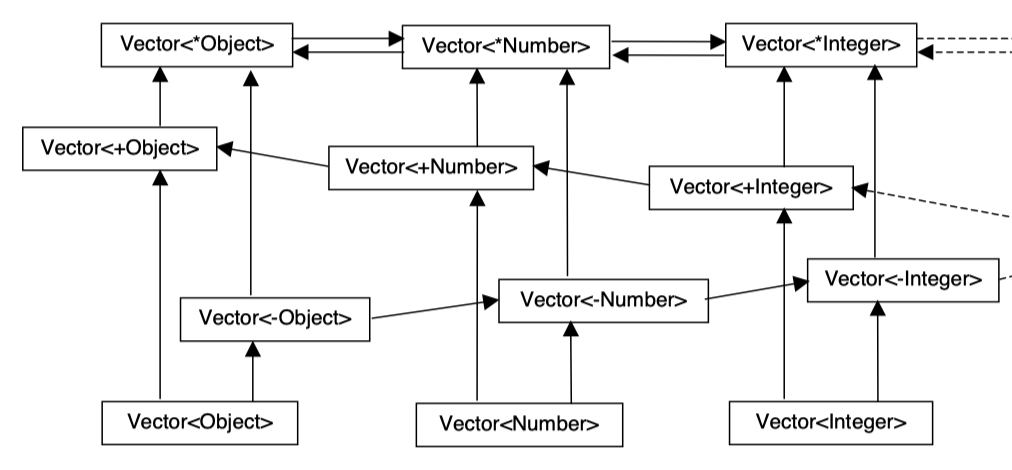
\includegraphics[scale=0.28]{img/subtype}
\end{center}

\end{frame}

\section{Type System}
\begin{frame}{Syntax}
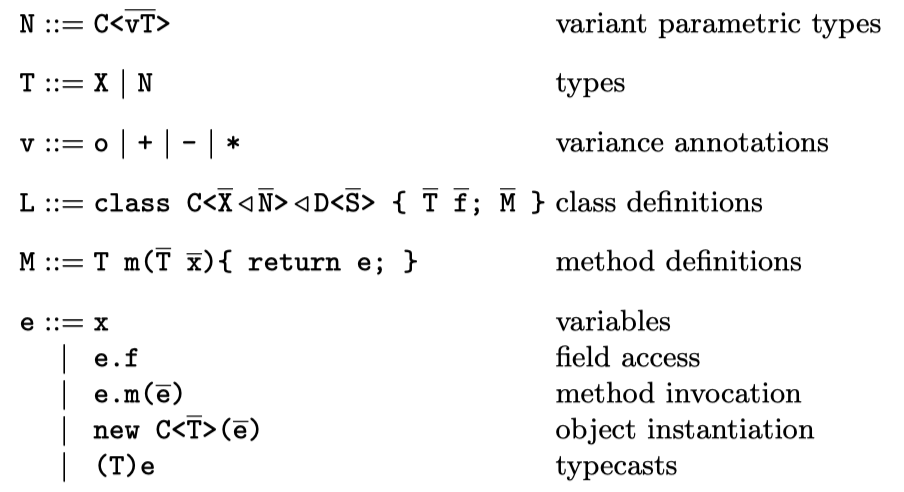
\includegraphics[scale=0.28]{img/syntax}
\end{frame}
\begin{frame}{Auxiliary functions}
\centering
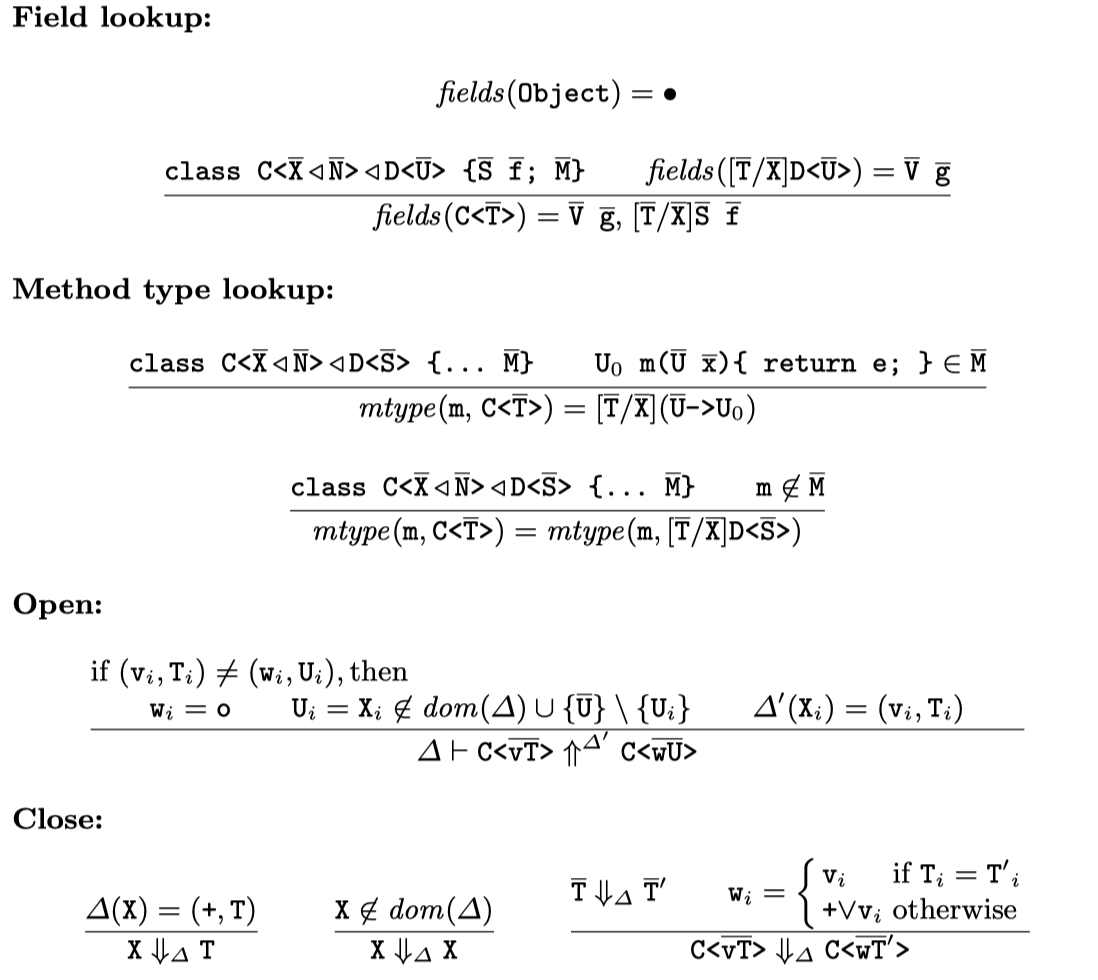
\includegraphics[scale=0.20]{img/type1}
\end{frame}
\begin{frame}{Judgments}
\centering
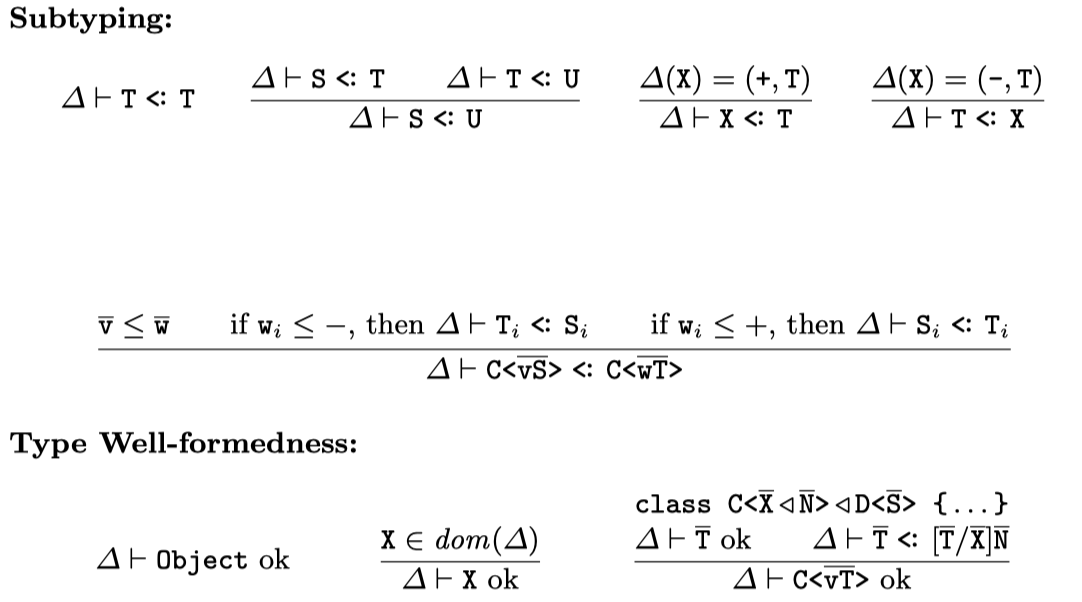
\includegraphics[scale=0.25]{img/type2}
\end{frame}
\begin{frame}{Typing}
\centering
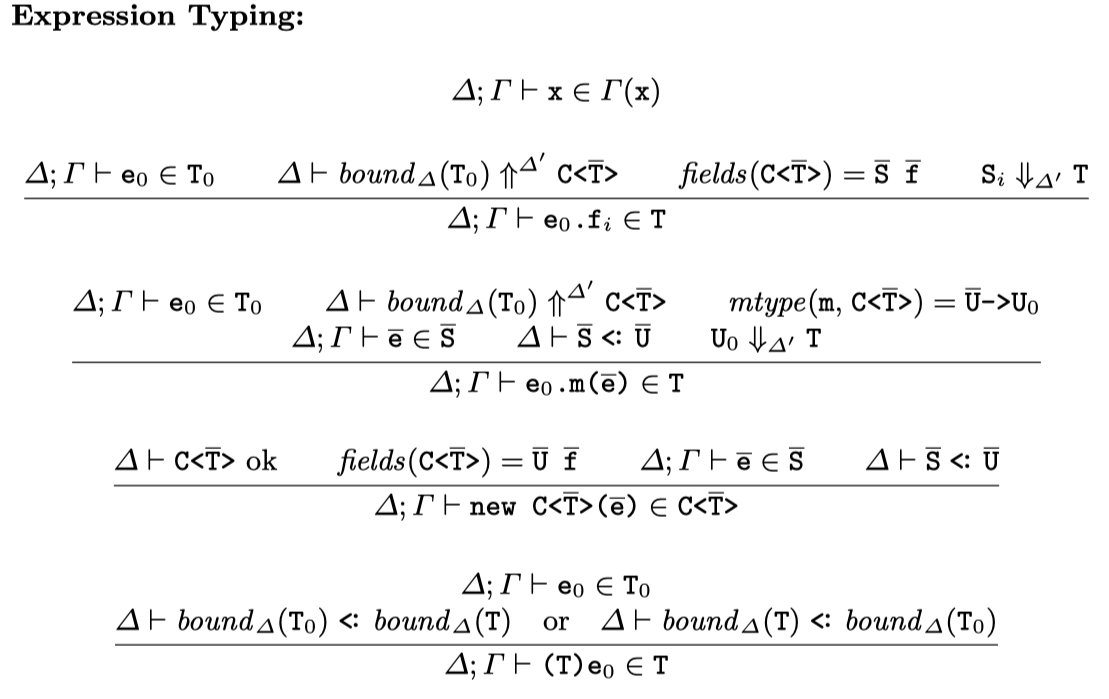
\includegraphics[scale=0.25]{img/type3}
\end{frame}

\begin{frame}{Final check}
\centering
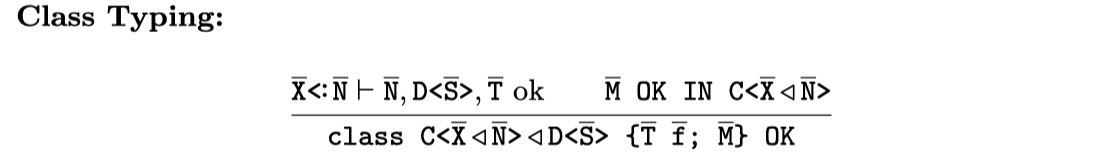
\includegraphics[scale=0.25]{img/type4}
\end{frame}











\end{document}